\documentclass[svgnames,11pt]{beamer}
\input{/home/tof/Documents/Cozy/latex-include/preambule_commun.tex}
\input{/home/tof/Documents/Cozy/latex-include/preambule_beamer.tex}
%\usepackage{pgfpages} \setbeameroption{show notes on second screen=left}
\author[]{Christophe Viroulaud}
\title{Chiffrement asymétrique\\RSA}
\date{\framebox{\textbf{Archi 23}}}
%\logo{}
\institute{Terminale - NSI}

\begin{document}
\begin{frame}
\titlepage
\end{frame}
\begin{frame}

    Le chiffrement asymétrique de Diffie-Hellman permet d'échanger des clés via un canal non sûr mais ne gère pas les problèmes liés à l'authentification des interlocuteurs.

\note{ En s'inspirant de ces travaux, \emph{Ron Rivest, Adi Shamir et Len Adleman} créent une méthode qui lève cette difficulté.}
\end{frame}
\begin{frame}
    \frametitle{}

    \begin{framed}
        \centering Comment authentifier avec certitude les participants?
    \end{framed}
\end{frame}
\section{Chiffrement RSA}
\subsection{Principe}
\begin{frame}
    \frametitle{Chiffrement RSA - Principe}
\begin{itemize}
    \item 1977: Ron Rivest, Adi Shamir et Len Adleman. 
    \item breveté en 1983; expiration du brevet en 2000.
    \item utilise \emph{des fonctions mathématiques à sens unique} (comme Diffie-Hellman)
    \item une paire de clés publique et privée.

\end{itemize}  
\begin{aretenir}[]
Une fonction à sens unique est une fonction mathématique facile à calculer mais pour laquelle il est très compliqué de retrouver l'antécédent d'une image.
\end{aretenir}
\end{frame}

\begin{frame}
    \frametitle{}

    \begin{aretenir}[]
    Le principe du protocole RSA s'inspire de la méthode de Diffie-Hellman:
        {\Large$$K_{priv}(K_{pub}(m))=K_{pub}(K_{priv}(m))=m$$}
    \end{aretenir}
\note{principe de Diffie-Hellman était différent: $f(f(x,y),z)=f(f(x,z),y)$}
\end{frame}
\newcommand{\puzzle}[3]{
    \draw[fill=white] (#1-0.6,#2) -- (#1-0.6,0.7+#2) -- (1+#1,0.7+#2) arc (220:-40:0.3) -- (3.1+#1,0.7+#2) -- (3.1+#1,#2) -- cycle;
    \node at(#1+1.25,0.35+#2){#3};
    }
\newcommand{\puzzlebis}[3]{
    \draw (#1-0.6,1.9+#2) -- (#1-0.6,0.7+#2) -- (1+#1,0.7+#2) arc (220:-40:0.3) -- (3.1+#1,0.7+#2) -- (3.1+#1,1.9+#2) -- cycle;
    \node at(#1+1.25,1.55+#2){#3};
    }
\subsection{Description}
\begin{frame}
    \frametitle{Description}

\begin{center}
    \begin{tikzpicture}[scale=0.85, transform shape]
        
        \node at(-4,0){Alice};
        \node at(0,0){Canal non sécurisé};
        \node at(4,0){Bob};
        \draw[dashed] (-2,0) -- (-2,-15) ;
        \draw[dashed] (2,0) -- (2,-15) ;

        \node[draw] at(0,-1){Étape 1};
        \puzzle{-5.2}{-3.2}{Clé publique};
        \puzzlebis{-5.2}{-3.2}{Clé privée};
        \node at(4,-2.5){Message};

    \end{tikzpicture}
\end{center}
\end{frame}

\begin{frame}
    \frametitle{}

\begin{center}
    \begin{tikzpicture}[scale=0.85, transform shape]
        
        \node at(-4,0){Alice};
        \node at(0,0){Canal non sécurisé};
        \node at(4,0){Bob};
        \draw[dashed] (-2,0) -- (-2,-15) ;
        \draw[dashed] (2,0) -- (2,-15) ;

        \node[draw] at(0,-1){Étape 1};
        \puzzle{-5.2}{-3.2}{Clé publique};
        \puzzlebis{-5.2}{-3.2}{Clé privée};
        \node at(4,-2.5){Message};


        \node[draw] at(0,-4){Étape 2};
        \draw[->,>=latex] (-4,-5.8) -- (4,-5.8);
        \puzzle{0}{-6.2}{Clé publique};
        \puzzlebis{-5.2}{-6.2}{Clé privée};
        \node at(4,-5.5){Message};

    \end{tikzpicture}
\end{center}
\end{frame}

\begin{frame}
    \frametitle{}

\begin{center}
    \begin{tikzpicture}[scale=0.85, transform shape]
        
        \node at(-4,-6){Alice};
        \node at(0,-6){Canal non sécurisé};
        \node at(4,-6){Bob};
        \draw[dashed] (-2,-6) -- (-2,-15) ;
        \draw[dashed] (2,-6) -- (2,-15) ;


        \node[draw] at(0,-7){Étape 3};
        \puzzle{3}{-9.2}{C\textbf{M}l\textbf{e}é \textbf{s}p\textbf{s}u\textbf{a}b\textbf{g}l\textbf{e}ique};
        \puzzlebis{-5.2}{-9.2}{Clé privée};


    \end{tikzpicture}
\end{center}
\end{frame}

\begin{frame}
    \frametitle{}

\begin{center}
    \begin{tikzpicture}[scale=0.85, transform shape]
        
        \node at(-4,-6){Alice};
        \node at(0,-6){Canal non sécurisé};
        \node at(4,-6){Bob};
        \draw[dashed] (-2,-6) -- (-2,-15) ;
        \draw[dashed] (2,-6) -- (2,-15) ;


        \node[draw] at(0,-7){Étape 3};
        \puzzle{3}{-9.2}{C\textbf{M}l\textbf{e}é \textbf{s}p\textbf{s}u\textbf{a}b\textbf{g}l\textbf{e}ique};
        \puzzlebis{-5.2}{-9.2}{Clé privée};

        \node[draw] at(0,-10){Étape 4};
        \draw[<-,>=latex] (-4,-11.8) -- (4,-11.8);
        \puzzle{-2}{-12.2}{C\textbf{M}l\textbf{e}é \textbf{s}p\textbf{s}u\textbf{a}b\textbf{g}l\textbf{e}ique};
        \puzzlebis{-5.2}{-12.2}{Clé privée};


    \end{tikzpicture}
\end{center}
\end{frame}

\begin{frame}
    \frametitle{}

\begin{center}
    \begin{tikzpicture}[scale=0.85, transform shape]
        
        \node at(-4,-6){Alice};
        \node at(0,-6){Canal non sécurisé};
        \node at(4,-6){Bob};
        \draw[dashed] (-2,-6) -- (-2,-15) ;
        \draw[dashed] (2,-6) -- (2,-15) ;


        \node[draw] at(0,-7){Étape 3};
        \puzzle{3}{-9.2}{C\textbf{M}l\textbf{e}é \textbf{s}p\textbf{s}u\textbf{a}b\textbf{g}l\textbf{e}ique};
        \puzzlebis{-5.2}{-9.2}{Clé privée};

        \node[draw] at(0,-10){Étape 4};
        \draw[<-,>=latex] (-4,-11.8) -- (4,-11.8);
        \puzzle{-2}{-12.2}{C\textbf{M}l\textbf{e}é \textbf{s}p\textbf{s}u\textbf{a}b\textbf{g}l\textbf{e}ique};
        \puzzlebis{-5.2}{-12.2}{Clé privée};

        \node[draw] at(0,-13){Étape 5};
        \puzzle{-5.2}{-15.2}{Message};
        \puzzlebis{-5.2}{-15.2}{};

    \end{tikzpicture}
\end{center}
\end{frame}
\begin{frame}
    \frametitle{}

    \begin{aretenir}[]
        Mathématiquement, la fonction respecte les règles suivantes:
        \begin{itemize}
            \item Il est impossible de deviner la clé privée en connaissant la clé publique.
            \item Il est impossible de deviner le message avec une seule des deux clés.
        \end{itemize}
    \end{aretenir}

\end{frame}

\subsection{kid RSA: formalisme mathématique}
\begin{frame}
    \frametitle{kid RSA}

    La création des clés suit un algorithme mathématique complexe. L'université de Rhode Island a produit une version simplifiée (à utilisation pédagogique) pour simuler le protocole.

\end{frame}
\begin{frame}
    \frametitle{}

    \begin{activite}
        \begin{enumerate}
            \item Découvrir l'algorithme \emph{kidrsa} sur la page \url{https://tinyurl.com/rsakid}
            \item Écrire la fonction \textbf{\texttt{creer\_nombre(a: int, b: int, a1: int, b1: int) $\rightarrow$ dict}} qui renvoie un dictionnaire contenant les clés privée et publique. Chaque clé sera un tuple.
            \item Écrire la fonction \textbf{\texttt{chiffrer(message: int, publique: tuple) $\rightarrow$ int}} qui encode \texttt{\textbf{message}} avec la clé publique (\emph{e, n}).
            \item Écrire la fonction \textbf{\texttt{dechiffrer(message\_chiffre: int, privee: tuple) $\rightarrow$ int}} qui déchiffre \texttt{\textbf{message\_chiffre}} avec la clé privée \emph{(d, n)}.
            \item Tester l'algorithme de chiffrage avec un entier (inférieur à n). Le message à chiffrer sera l'entier 538.
        \end{enumerate}
        \end{activite}

\end{frame}
\begin{frame}
    \frametitle{Correction}

    \begin{center}
        \lstinputlisting[firstline=10 ,lastline=20,basicstyle=\small\ttfamily,xleftmargin=0.2em,xrightmargin=-3.5em ]{"scripts/kidrsa.py"}
    \captionof{code}{Alice crée ses clés}
    \end{center}

\end{frame}
\begin{frame}
    \frametitle{Correction}

    \begin{center}
        \lstinputlisting[firstline=23 ,lastline=32,basicstyle=\small\ttfamily,xleftmargin=0.2em,xrightmargin=0em  ]{"scripts/kidrsa.py"}
    \captionof{code}{Bob chiffre son message avec la clé publique d'Alice}
    \end{center}

\end{frame}
\begin{frame}
    \frametitle{Correction}

    \begin{center}
        \lstinputlisting[firstline=35 ,lastline=44,basicstyle=\small\ttfamily,xleftmargin=0.2em,xrightmargin=0em  ]{"scripts/kidrsa.py"}
    \captionof{code}{Alice déchiffre le message de Bob avec sa clé privée}
    \end{center}

\end{frame}
\begin{frame}[fragile]
    \frametitle{}

    
\begin{center}
\begin{lstlisting}[language=Python , basicstyle=\ttfamily\small, xleftmargin=0.2em, xrightmargin=0em]
>>> cles = creer_nombre(9, 11, 5, 8)
>>> cles
{'publique': (499, 4048), 'privee': (795, 4048)}

>>> s = chiffrer(538, cles["publique"])
>>> s
1294

>>> e = dechiffrer(s, cles["privee"])
>>> e
538
\end{lstlisting}
\end{center}
\end{frame}
\begin{frame}
    \frametitle{}

\begin{center}
    Pour l'instant, l'algorithme RSA ne fait rien de plus que celui de Diffie-Hellman. Le problème de l'authentification n'est toujours pas résolu.

\end{center}

\end{frame}
\section{Authentification des participants}
\begin{frame}
    \frametitle{Authentification des participants}
\begin{aretenir}[]
Pour certifier l'identité des individus, il faut qu'un \textbf{tiers de confiance} (Nestor) intervienne.
\end{aretenir}
\note{Nestor = neutre = version francophone de Trent (trusted)}
\end{frame}


\begin{frame}
    \frametitle{}

\begin{center}
    \begin{tikzpicture}[scale=0.9, transform shape]
        
        \node at(-5,0){Alice};
        \node at(0,0){Nestor};
        \draw[dashed] (-3,0) -- (-3,-8) ;
        \draw[dashed] (3,0) -- (3,-8) ;

        \node[draw] at(0,-1){Étape 1};
        \node at(-5,-3){$K^{Alice}_{pub}$};
        \node at(0,-2){$K^{Nestor}_{priv}$};
        \node at(0,-3){$K^{Nestor}_{pub}$};

    \end{tikzpicture}
    \captionof{figure}{Le tiers de confiance crée un couple de clés privée/publique.}
\end{center}
\note{Le tiers de confiance crée un couple privé/publique; On ne s'intéresse qu'à la clé publique de Alice = celle qui va être transmise.}
\end{frame}

\begin{frame}
    \frametitle{}

\begin{center}
    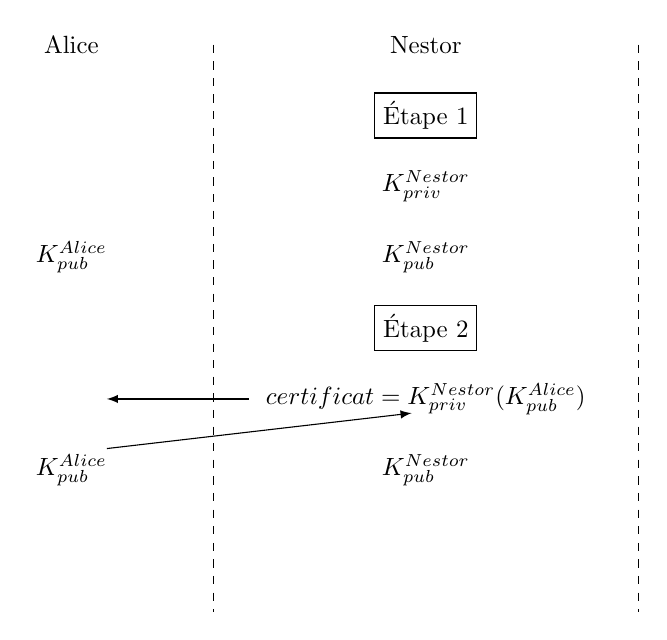
\begin{tikzpicture}[scale=0.9, transform shape]
        
        \node at(-5,0){Alice};
        \node at(0,0){Nestor};
        \draw[dashed] (-3,0) -- (-3,-8) ;
        \draw[dashed] (3,0) -- (3,-8) ;

        \node[draw] at(0,-1){Étape 1};
        \node at(-5,-3){$K^{Alice}_{pub}$};
        \node at(0,-2){$K^{Nestor}_{priv}$};
        \node at(0,-3){$K^{Nestor}_{pub}$};

        \node[draw] at(0,-4){Étape 2};
        \draw[<-,>=latex] (-4.5,-5) -- (-2.5,-5);
        \draw[->,>=latex] (-4.5,-5.7) -- (-0.2,-5.2);
        \node at(-5,-6){$K^{Alice}_{pub}$};
        \node at(0,-5){$certificat=K^{Nestor}_{priv}(K^{Alice}_{pub})$};
        \node at(0,-6){$K^{Nestor}_{pub}$};

    \end{tikzpicture}
    \captionof{figure}{\centering Nestor chiffre la clé publique d'Alice avec sa clé privée: il crée un \textbf{certificat}.}
\end{center}
\note{Nestor chiffre la clé publique d'Alice avec sa clé privée $\rightarrow$ certificat.}
\end{frame}
\begin{frame}
    \frametitle{}

\begin{center}
    \begin{tikzpicture}[scale=0.9, transform shape]
        
        \node at(-4,-6){Alice};
        \node at(0,-6){Nestor};
        \node at(4,-6){Bob};
        \draw[dashed] (-2,-6) -- (-2,-12) ;
        \draw[dashed] (2,-6) -- (2,-12) ;

        \node[draw] at(0,-7){Étape 3};
        \draw[->,>=latex] (-1.5,-8) -- (4.5,-8);
        \draw[->,>=latex] (-2,-9) -- (4.5,-8);

        \node at(-4,-8){$certificat=K^{Nestor}_{priv}(K^{Alice}_{pub})$};
        \node at(-5,-9){$K^{Alice}_{pub}$};
        \node at(0,-9.3){$K^{Nestor}_{pub}$};


    \end{tikzpicture}
    \captionof{figure}{Alice envoie le certificat et sa clé publique en clair.}
\end{center}
\note{Alice envoie le certificat et sa clé publique en clair}
\end{frame}
\begin{frame}
    \frametitle{}

\begin{center}
    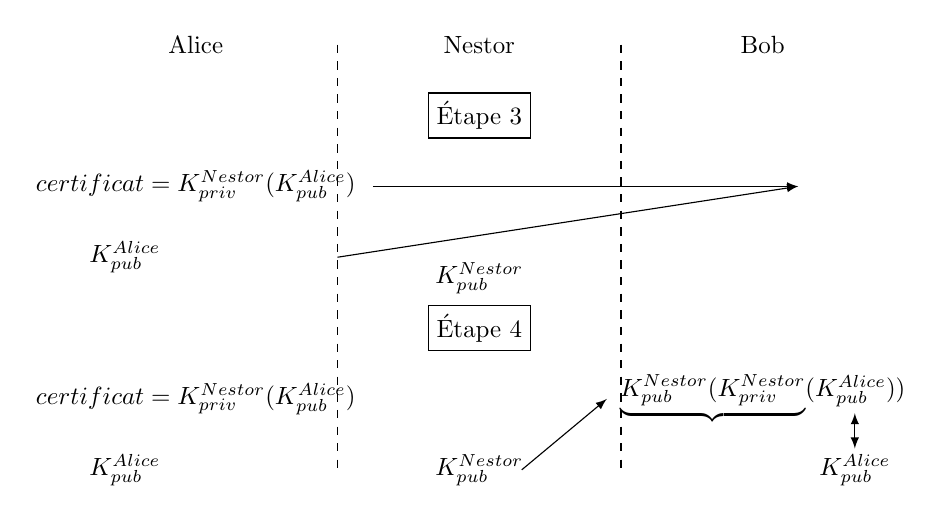
\begin{tikzpicture}[scale=0.9, transform shape]
        
        \node at(-4,-6){Alice};
        \node at(0,-6){Nestor};
        \node at(4,-6){Bob};
        \draw[dashed] (-2,-6) -- (-2,-12) ;
        \draw[dashed] (2,-6) -- (2,-12) ;

        \node[draw] at(0,-7){Étape 3};
        \draw[->,>=latex] (-1.5,-8) -- (4.5,-8);
        \draw[->,>=latex] (-2,-9) -- (4.5,-8);

        \node at(-4,-8){$certificat=K^{Nestor}_{priv}(K^{Alice}_{pub})$};
        \node at(-5,-9){$K^{Alice}_{pub}$};
        \node at(0,-9.3){$K^{Nestor}_{pub}$};


        \node[draw] at(0,-10){Étape 4};
        \draw[->,>=latex] (0.6,-12) -- (1.8,-11);
        \draw[<->,>=latex] (5.3,-11.2) -- (5.3,-11.7);
        \node at(-4,-11){$certificat=K^{Nestor}_{priv}(K^{Alice}_{pub})$};
        \node at(-5,-12){$K^{Alice}_{pub}$};
        \node at(0,-12){$K^{Nestor}_{pub}$};

        \node at(4,-11){$\underbrace{K^{Nestor}_{pub}(K^{Nestor}_{priv}}(K^{Alice}_{pub}))$};
        \node at(5.3,-12){$K^{Alice}_{pub}$};

    \end{tikzpicture}
    \captionof{figure}{\centering À l'aide de la clé publique de Nestor, Bob déchiffre la clé publique d'Alice (le certificat) et la compare à la clé publique fournie en clair.}
\end{center}
\note[item]{pas possible avec Diffie car $f(f(x,y),z)=f(f(x,z),y)$ $\leftarrow$ non réversibilité des pots de peinture}
\end{frame}

\section{Sécuriser l'accès à un site web}
\subsection{Associer les protocoles}
\begin{frame}
    \frametitle{Sécuriser l'accès à un site web}

    L'algorithme RSA:
    \begin{itemize}
        \item<1-> \textbf{avantage: }permet de sécuriser les données
        \item<2-> \textbf{avantage:} permet d'authentifier les participants.
        \item<3-> \textbf{inconvénient: } est très coûteux en temps de calcul.
    \end{itemize}


\end{frame}

\begin{frame}
    \frametitle{}
    \begin{aretenir}[]
        On mettra à profit les avantages de chaque type de chiffrement:
        \begin{itemize}
            \item Le chiffrement symétrique, rapide, sera utilisé pour chiffrer les données avec une \emph{clé de chiffrement symétrique}.
            \item Le chiffrement asymétrique, permettant d'authentifier les participants, sera utilisé pour transmettre la clé de chiffrement symétrique.
        \end{itemize}
        \end{aretenir}
    
\note{RSA = authentification; symétrique ou Diffie-Hellman pour chiffrement}
\end{frame}
\subsection{Autorité de certification}
%différents niveaux
\begin{frame}
    \frametitle{Autorité de certification}

    Une autorité de certification peut être:
\begin{itemize}
    \item un état,
    \item une entreprise spécialisée,
    \item une association à but non lucratif (Let's Encrypt).
\end{itemize}
\note{règles très strictes, audités régulièrement}

\end{frame}
\begin{frame}
    \frametitle{}

    Les navigateurs possèdent une copie des clés publiques de ces autorités de certification.

\begin{center}
\centering
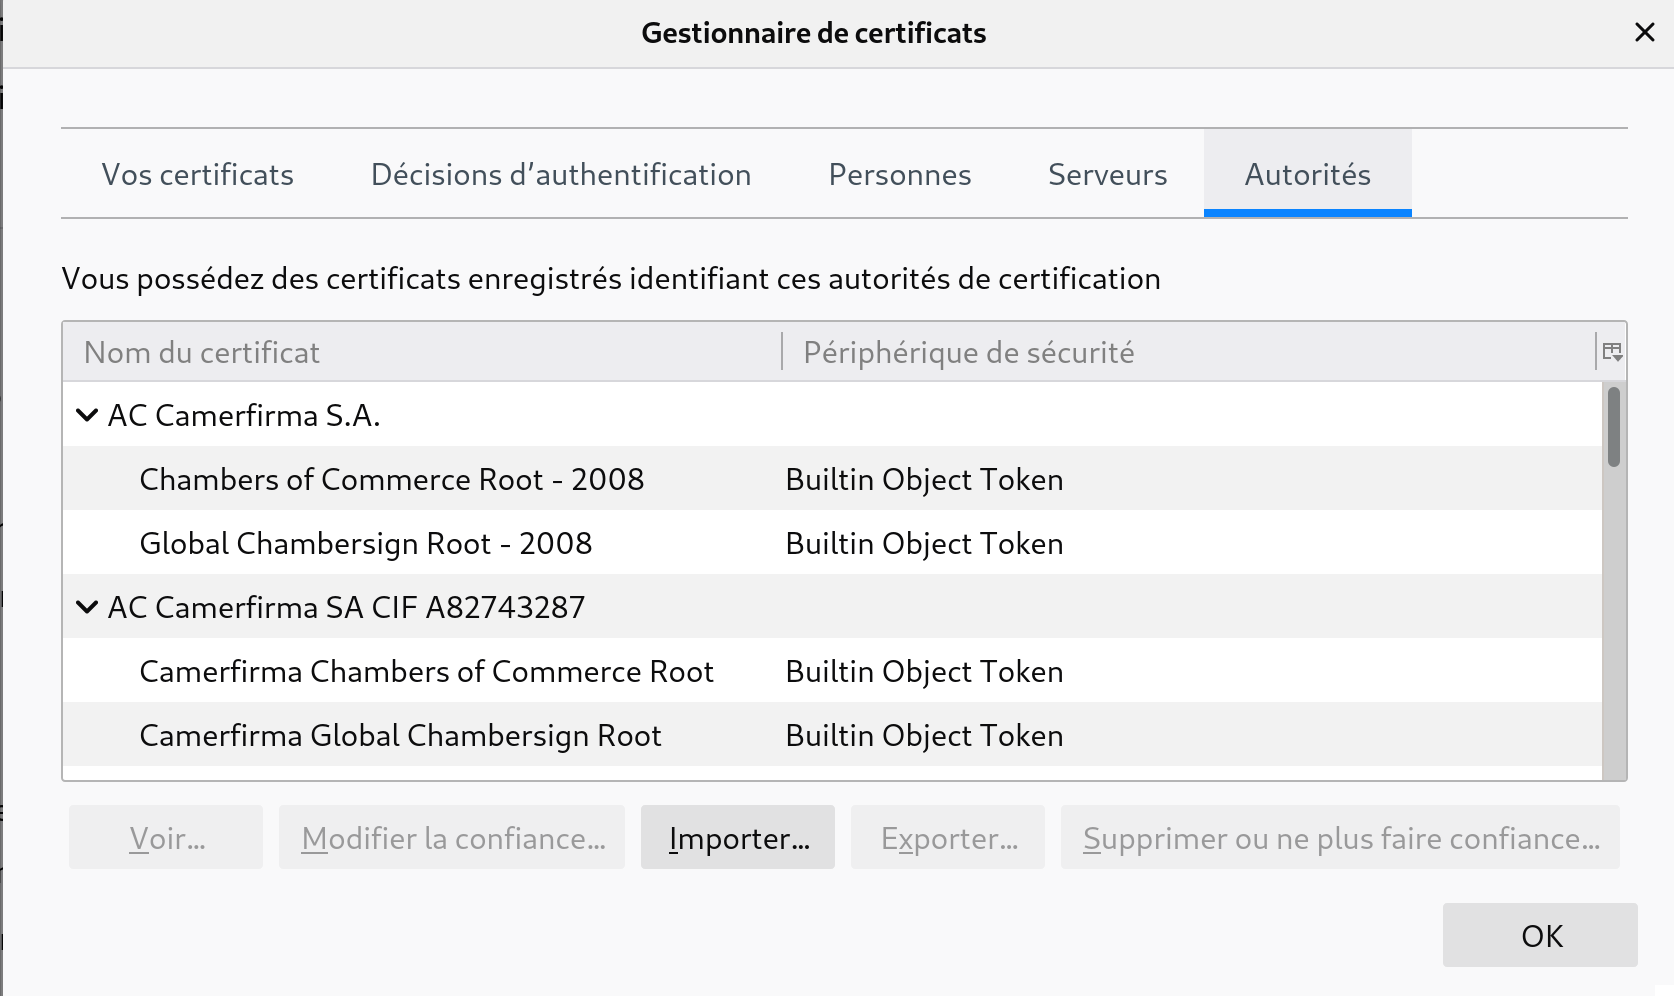
\includegraphics[width=9cm]{ressources/certificats.png}
\captionof{figure}{Firefox/préférences/vie privée et sécurité/certificats}
\label{IMG}
\end{center}


\end{frame}
\begin{frame}
    \frametitle{}

    \begin{aretenir}[Hors programme]
        En pratique, l'autorité de certification ne signe pas la clé publique entière du site (2048 ou 4096 bits) mais sa somme de contrôle calculée (256 bits) par une fonction de hachage (souvent sha256).
    \end{aretenir}

\end{frame}
\subsection{Protocole https}
\begin{frame}
    \frametitle{Protocole https}
    Le protocole \emph{https} ajoute une couche \emph{TLS (Transport Layer Security)} au protocole \emph{http} existant.


    \note[item]{SSL (Secure Sockets Layer) = ancêtre TLS (sécurité de la couche de transport)}

\end{frame}
\begin{frame}
    \frametitle{}

    \begin{center}
        \begin{tikzpicture}[scale=0.83, transform shape]
            
            \node at(-5,0){Client};
            \node at(0,0){Internet};
            \node at(5,0){Serveur};
            \draw[dashed] (-3,0) -- (-3,-7) ;
            \draw[dashed] (3,0) -- (3,-7) ;
    
            \draw[->,>=latex, dashed] (-5,-1) -- (5,-2) node[sloped, midway, fill=white]{Hello};
            
        \end{tikzpicture}
        \captionof{figure}{\centering \textbf{Hello: }Le navigateur envoie son intention de se connecter et diverses informations techniques.}
    \end{center}
\note[item]{Hello: infos techniques (algo de chiffrement qu'il peut utiliser)}
\end{frame}
\begin{frame}
    \frametitle{}

    \begin{center}
        \begin{tikzpicture}[scale=0.83, transform shape]
            
            \node at(-5,0){Client};
            \node at(0,0){Internet};
            \node at(5,0){Serveur};
            \draw[dashed] (-3,0) -- (-3,-7) ;
            \draw[dashed] (3,0) -- (3,-7) ;
    
            \draw[->,>=latex, dashed] (-5,-1) -- (5,-2) node[sloped, midway, fill=white]{Hello};
            \draw[->,>=latex, dashed] (5,-2) -- (-5,-3) node[sloped, midway, fill=white]{Certificat};
            
        \end{tikzpicture}
        \captionof{figure}{\centering \textbf{Certificat:} Le serveur envoie son certificat (sa clé publique signée par la clé privée d'une autorité).}
    \end{center}

\end{frame}
\begin{frame}
    \frametitle{}

    \begin{center}
        \begin{tikzpicture}[scale=0.83, transform shape]
            
            \node at(-5,0){Client};
            \node at(0,0){Internet};
            \node at(5,0){Serveur};
            \draw[dashed] (-3,0) -- (-3,-7) ;
            \draw[dashed] (3,0) -- (3,-7) ;
    
            \draw[->,>=latex, dashed] (-5,-1) -- (5,-2) node[sloped, midway, fill=white]{Hello};
            \draw[->,>=latex, dashed] (5,-2) -- (-5,-3) node[sloped, midway, fill=white]{Certificat};
            \node at(-5,-3.5){$K^{Nestor}_{pub}+certificat$};
        \end{tikzpicture}
        \captionof{figure}{\centering \textbf{Authentification: }Le client utilise la clé publique de l'autorité pour déchiffrer le certificat et compare le résultat avec la clé publique du site.}
    \end{center}

\end{frame}
\begin{frame}
    \frametitle{}

    \begin{center}
        \begin{tikzpicture}[scale=0.83, transform shape]
            
            \node at(-5,0){Client};
            \node at(0,0){Internet};
            \node at(5,0){Serveur};
            \draw[dashed] (-3,0) -- (-3,-7) ;
            \draw[dashed] (3,0) -- (3,-7) ;
    
            \draw[->,>=latex, dashed] (-5,-1) -- (5,-2) node[sloped, midway, fill=white]{Hello};
            \draw[->,>=latex, dashed] (5,-2) -- (-5,-3) node[sloped, midway, fill=white]{Certificat};
            \node at(-5,-3.5){$K^{Nestor}_{pub}+certificat$};
            \node at(-5,-4.3){$K^{site}_{pub}$};
    
            \draw[->,>=latex, dashed] (-5,-5) -- (5,-6) node[sloped, midway, fill=white]{clé de session};
    
        \end{tikzpicture}
        \captionof{figure}{\textbf{Clé de session: }Le client et le serveur se mettent d'accord sur un protocole d'échange (symétrique, Diffie-Hellman): le client peut communiquer sa clé de manière sécurisée grâce à la clé publique authentifiée du site.}
    \end{center}

\end{frame}
\begin{frame}
    \frametitle{}
    \begin{center}
        \begin{tikzpicture}[scale=0.83, transform shape]
            
            \node at(-5,0){Client};
            \node at(0,0){Internet};
            \node at(5,0){Serveur};
            \draw[dashed] (-3,0) -- (-3,-7) ;
            \draw[dashed] (3,0) -- (3,-7) ;
    
            \draw[->,>=latex, dashed] (-5,-1) -- (5,-2) node[sloped, midway, fill=white]{Hello};
            \draw[->,>=latex, dashed] (5,-2) -- (-5,-3) node[sloped, midway, fill=white]{Certificat};
            \node at(-5,-3.5){$K^{Nestor}_{pub}+certificat$};
            \node at(-5,-4.3){$K^{site}_{pub}$};
    
            \draw[->,>=latex, dashed] (-5,-5) -- (5,-6) node[sloped, midway, fill=white]{clé de session};
    
            \draw[<->,>=latex] (-5,-7) -- (5,-7) node[sloped, midway, fill=white]{échanges sécurisés};
        \end{tikzpicture}
        \captionof{figure}{\textbf{Échanges: }Le client et le serveur échangent de manière sécurisée.}
    \end{center}
    

\end{frame}
\subsection{Informations techniques}
\begin{frame}
    \frametitle{Informations techniques}

    \begin{center}
    \centering
    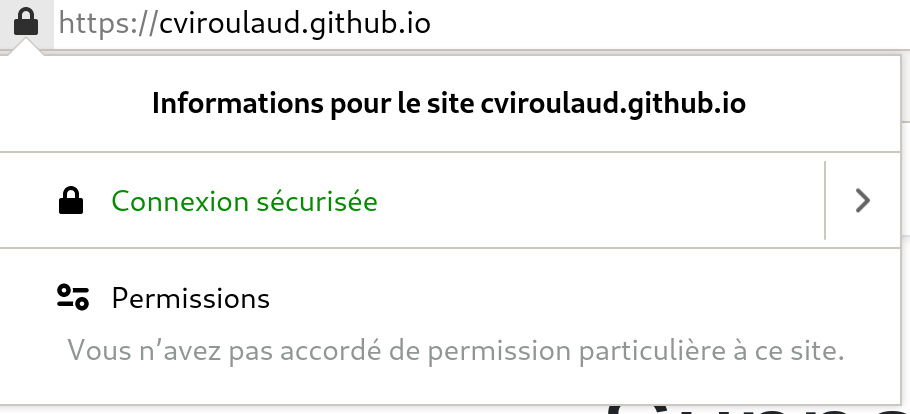
\includegraphics[width=8cm]{ressources/cadenas.png}
    \captionof{figure}{Le cadenas atteste des échanges sécurisés}
    \label{IMG}
    \end{center}

\end{frame}
\begin{frame}
    \frametitle{}

    \begin{center}
    \centering
    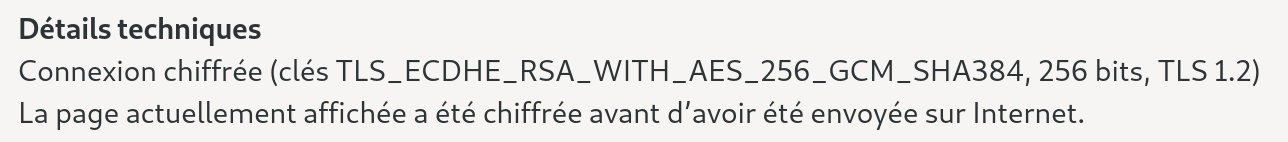
\includegraphics[width=10.5cm]{ressources/chiffrement.png}
        TLS\_ECDHE\_RSA\_WITH\_AES\_256\_GCM\_SHA384, 256bits, TLS 1.2
    \end{center}
\begin{itemize}
    \item Protocole \textbf{TLS} (Transport Layer Security)
    \note[item]{plutôt que SSL Secure Sockets Layer}
    \item Algorithme d’échange de clés : \textbf{ECDHE} (Elliptic Curve Diffie-Hellman Ephemeral)
    \item Algorithme d’authentification : \textbf{RSA}
    \item Algorithme de chiffrement (symétrique) par bloc : \textbf{AES 256bits} (Advanced Encryption Standard) en mode GCM (Galois/Counter Mode)
    \item Algorithme de code d’authentification de message : \textbf{SHA384} (création de la somme de contrôle de la clé)
\end{itemize}
\end{frame}
\end{document}